\documentclass[11pt]{beamer}
\usetheme{Warsaw}
\usepackage[utf8]{inputenc}
\usepackage{amsmath}
\usepackage{amsfonts}
\usepackage{amssymb}
\usepackage{graphicx}
\usepackage{verbatim}
\usepackage{fancyvrb}
\RecustomVerbatimCommand{\VerbatimInput}{VerbatimInput}%
{fontsize=\footnotesize}
\author{Jupiter Subgroup}
\title{Introduction to Making Documents with \LaTeX}
%\setbeamercovered{transparent} 
%\setbeamertemplate{navigation symbols}{} 
%\logo{} 
%\institute{} 
%\date{} 
%\subject{} 
\begin{document}

\begin{frame}
\titlepage
\end{frame}

%\begin{frame}
%\tableofcontents
%\end{frame}

%
%	Introduction
%
\begin{frame}{Introduction}
\begin{columns}
	\begin{column}{6cm}
		\underline{What \LaTeX{} is}
		\begin{itemize}
			\item	A cross-platform typesetting environment
			\item 	Best way to produce aesthetically pleasing, logically coherent documents, especially when dealing with mathematical equations
			\item 	Free and customizable
		\end{itemize}
	\end{column}
		\begin{column}{5cm}
		\underline{What \LaTeX{} isn't}
		\begin{itemize}
			\item WYSIWYG (What You See is What You Get)
				\begin{itemize}
					\item MS Word, LibreOffice
				\end{itemize}
			\item Bloated memory hog
		\end{itemize}
	\end{column}
	\end{columns}
\end{frame}

%
%	How it works
%
\begin{frame}{How it Works}
\begin{enumerate}
	\item The \TeX{} typesetting engine reads a plain text file, usually written using \LaTeX{} (a set of \TeX{} macros) \\
	\only<1>{\VerbatimInput{hello.tex}} 
	\item<2-> Produces a readable, formatted document image (.dvi) \\
		\only<2>{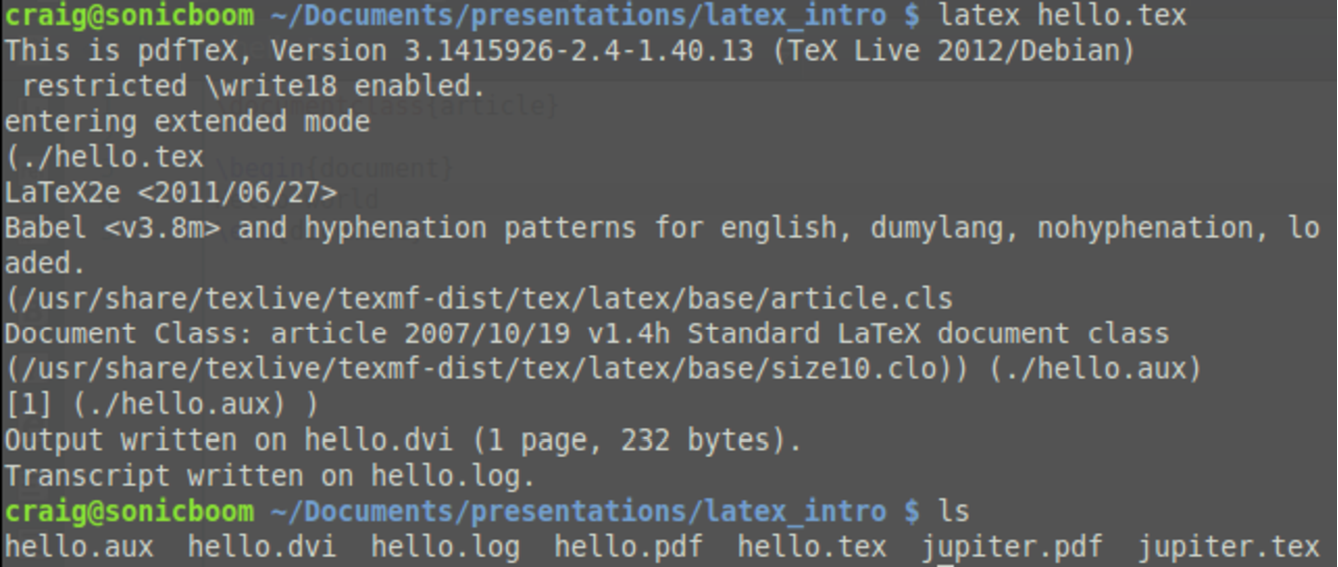
\includegraphics[scale=0.3]{hello_cli}}
	\item<3-> Convert to pdf (or straight to pdf using pdflatex)\\
			\only<3>{
\includegraphics[scale=.3]{hello}}
\end{enumerate}
\only<4> {Separates design from content $\rightarrow$ enhanced logical structure}
\end{frame}

%
%	What you need
%
\begin{frame}{What you Need}
\begin{enumerate}
	\item Text editor or IDE
	\begin{itemize}
		\item Texmaker, Vim/Emacs/gedit with plugins, Notepad++, Sublime
		\item Look for built-in output viewer, code completion \\
		\only<1>{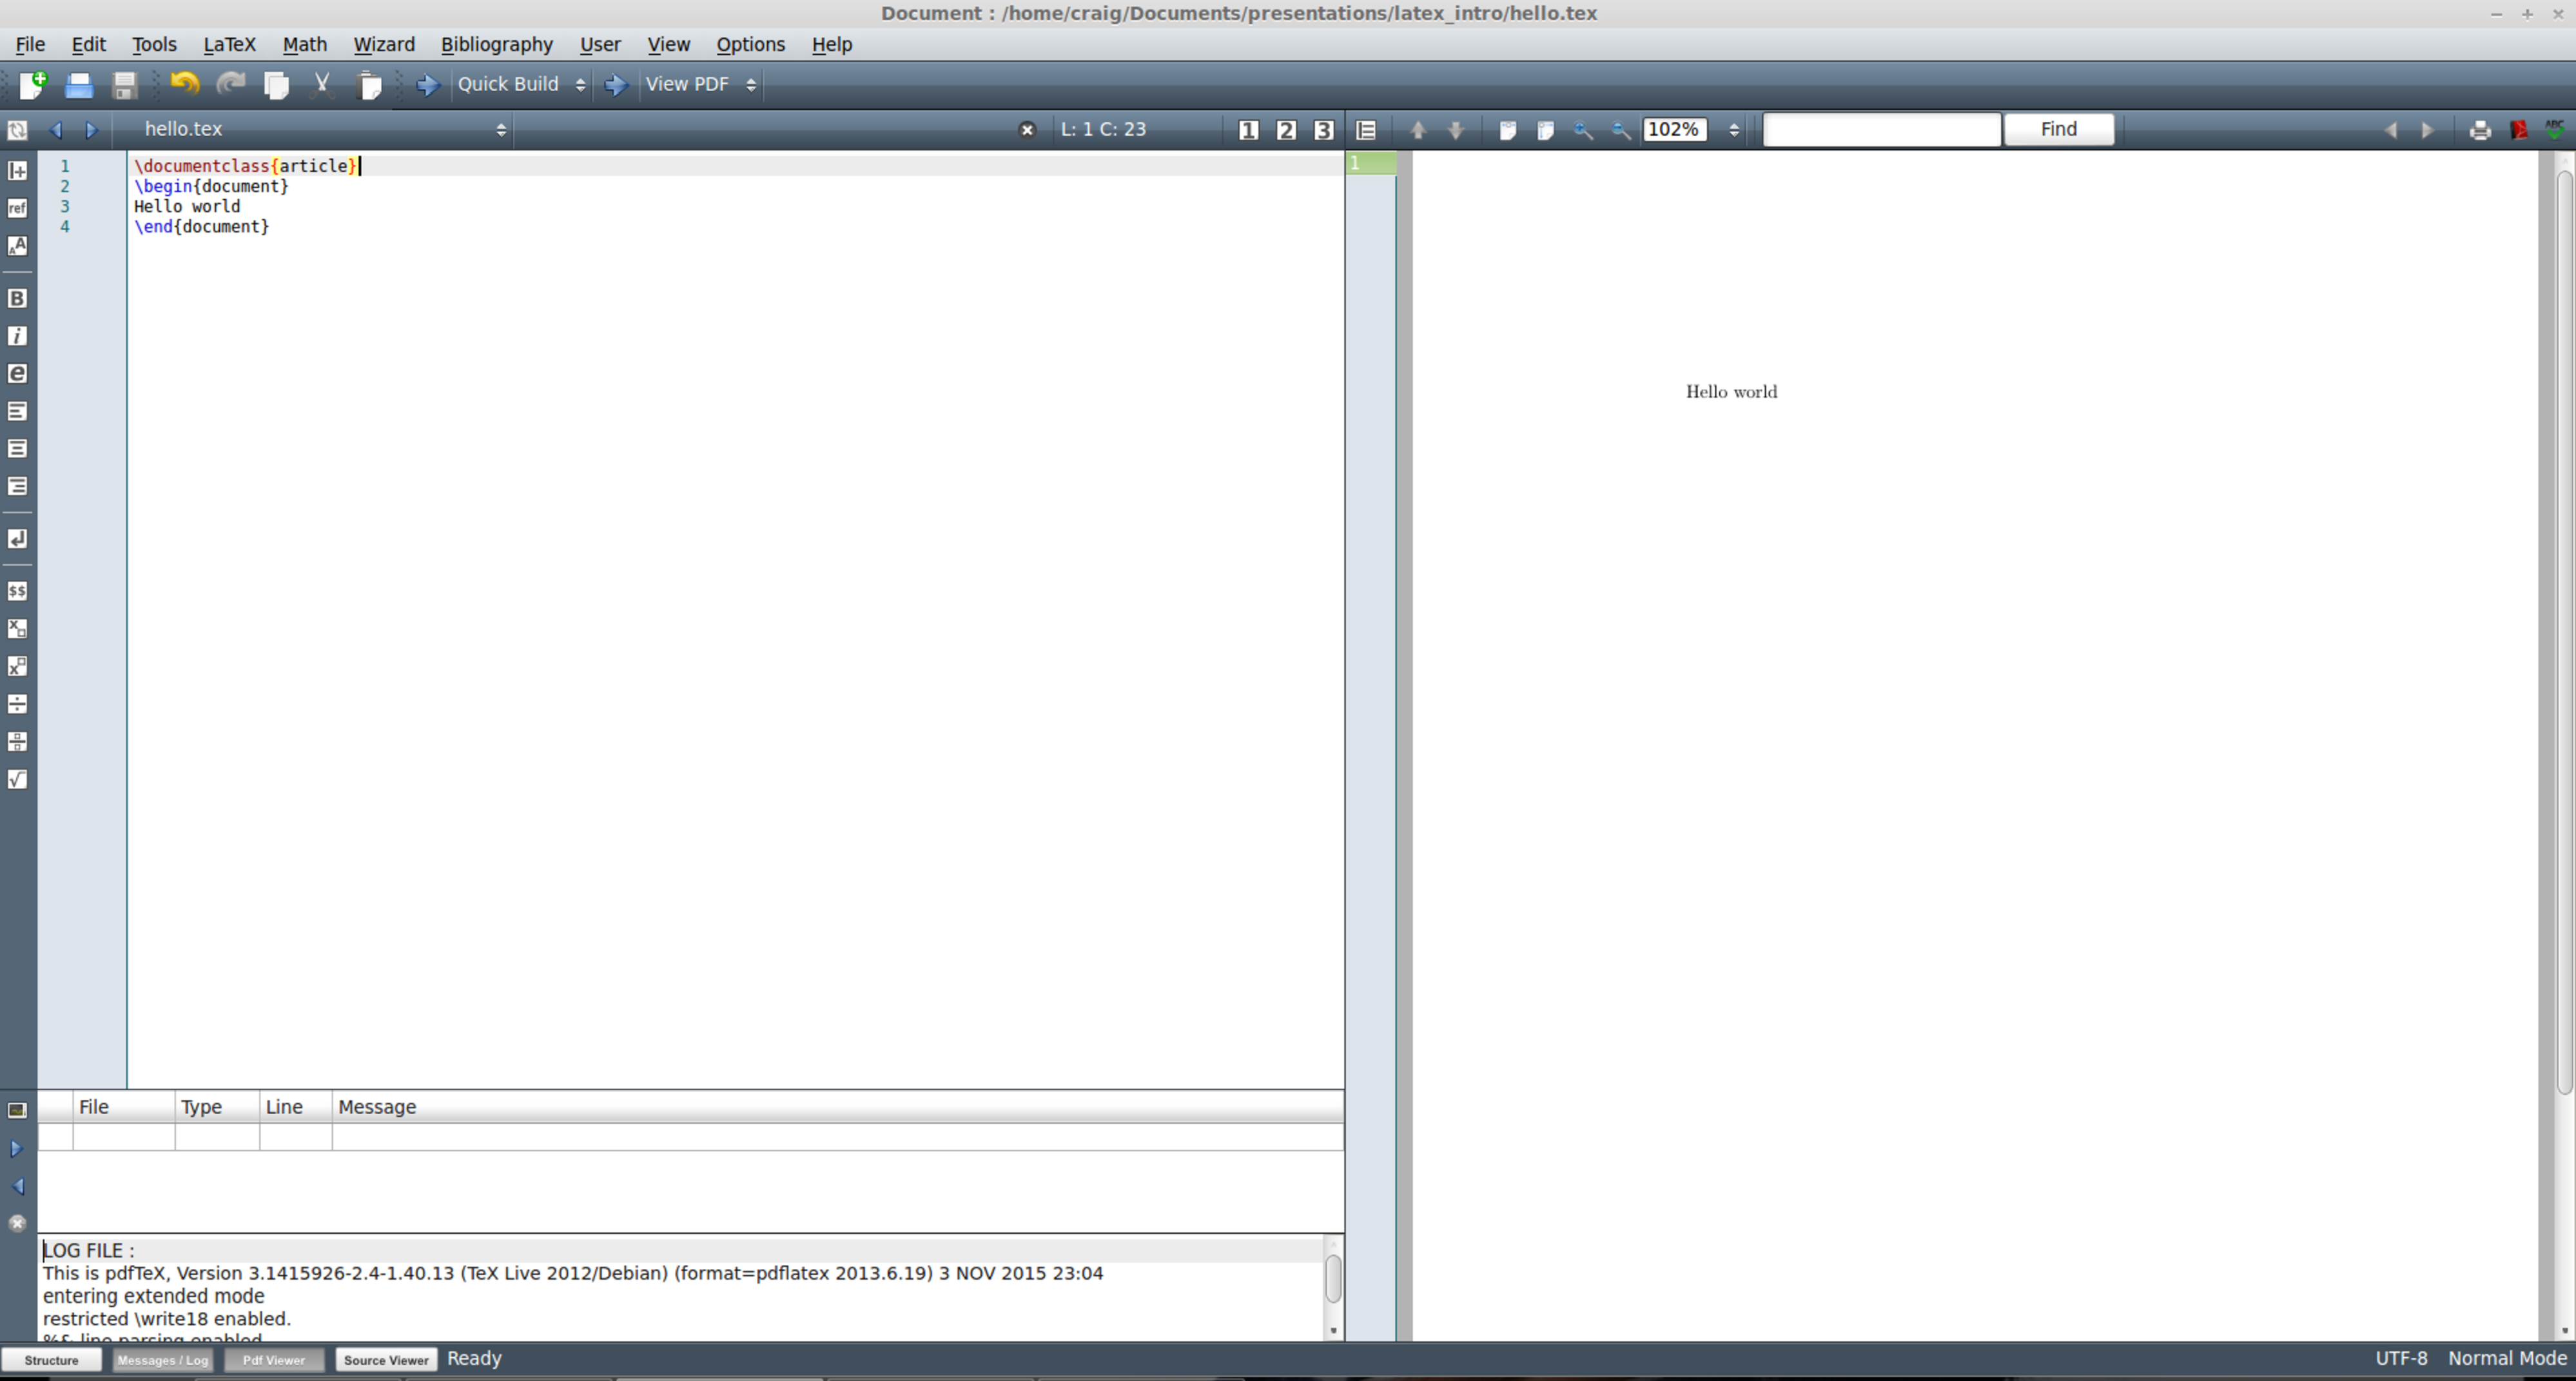
\includegraphics[scale=0.1]{texmaker}}
	\end{itemize}
	\item<2> Sane \LaTeX{} installation
	\begin{itemize}
		\item Windows - MikTeX
		\item Mac - MacTeX
		\item Linux - texlive
	\end{itemize}
\end{enumerate}
\end{frame}

%
% 	Special Characters
%
\begin{frame}{Special Characters, commands, and comments}
\begin{itemize}
	\item Special characters
	\begin{itemize}
		\item tells \LaTeX{} to do something, won't print like you intend
		\item \# \$ \% \^{} \& \_ \{ \} \~{}
\textbackslash
	\end{itemize}
	\item \LaTeX commands
	\begin{itemize}
		\item Start with a \textbackslash, i.e. \textbackslash backslash, \textbackslash alpha$\rightarrow \alpha$
	\end{itemize}
	\item Comment lines with \%
\end{itemize}
\end{frame}

%
% 	File Structure
%
\section{File Structure and Layout}
\begin{frame}{Input file structure and layout}
\begin{itemize}
	\item	Preamble
	\begin{itemize}
		\item	Contains all formatting directions and information not directly related to content
		\item Authors, date, institutions, title, external packages \\
		\only<1>{\VerbatimInput{headerexample.tex}}
	\end{itemize}
\end{itemize}
\end{frame}

%
% 	Packages
%
\begin{frame}{Packages and external files}
http://www.howtotex.com/packages/9-essential-latex-packages-everyone-should-use/
\end{frame}

%
% 	Typesetting
%
\section{Typesetting}
\begin{frame}{Typesetting}
paragraphs, line and page breaks, hyphenation, sections, chapters, alignment, itemize, enumerate, font sizes (table 6.3, 6.4)
\end{frame}

%
% 	File Structure
%
\begin{frame}{Some useful commands and characters}
emph, bold, under, degree, tilde, quotation, \"{o}, A$^{n}$, $\alpha_i$
\end{frame}

%
% 	File Structure
%
\begin{frame}{Some useful environments}
verbatim, tabular
\end{frame}

%
% 	Types of formulae
%
\section{Mathematical Formulae}
\begin{frame}{Mathematical Formulae}
AMS math, inline, single line display (numbered/unnumbered), multiple line display
\end{frame}

%
% 	Useful commands
%
\begin{frame}{Some useful commands}
Greek, super and sub script, sum (substack), integral, product operators, dots, frac, predefined functions, partial
\end{frame}

%
% 	Matrices
%
\begin{frame}{Arrays and matrices}
uses array environment for arrays, amsmath uses matrix environments
\end{frame}

%
% 	File Structure
%
\begin{frame}{Graphics}
use graphicx package (options), no real standard find what works, figure env. center, caption, includegraphics, remove extensions to avoid conflict b/w latex pdflatex
\end{frame}

%
% 	Bibliography
%
\begin{frame}{Bibliographies}
Use BibTeX, keep main bib file w/ consistent naming convention, bibliography command at end, bibliographystyle at beginning
\end{frame}

%
% 	Cross referencing
%
\begin{frame}{Cross referencing and citation}
Cleveref package, cite, ref, naming labels
\end{frame}

%
% 	Custom Commands
%
\begin{frame}{Custom commands}
newcommand-name, num of args, definition, hashtag w/ number for arguments, bra, ket, braket, 2x2 matrix \\
newenvironment, renewenvironment to override existing commands
\end{frame}

%
% 	Chemistry specific 
%
\begin{frame}{Chemistry specific packages}
https://www.ctan.org/topic/chemistry, chemfig-rings, rxn, achemso
\end{frame}

%
% 	Putting it all together
%
\begin{frame}{Putting it all together}
Keep a universal header, bib, and main document template. Copy and edit as needed. Example file with header, equations, cross reference, citations, and sections
\end{frame}

%
%	Resources
%
\begin{frame}{Resources}
lshort, ctan, http://www.xm1math.net/texmaker/
\end{frame}


\end{document}